
\begin{figure}[!htbp]
    \begin{centering}
        \subfloat[Runtime in minutes for correcting 25kb Matrix]
        {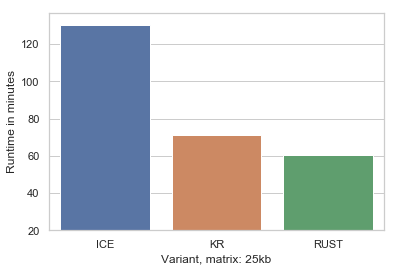
\includegraphics[scale=0.9]{figures/results/runtime_25}} \\
        % \caption[Correction time of 25kb]
        % {\textbf{Runtime in minutes} for correcting the 25kb matrix.}
        \subfloat[Runtime in minutes for correcting 50kb Matrix]
        {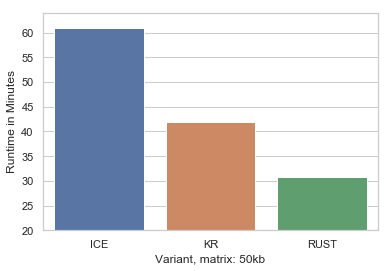
\includegraphics[scale=0.9]{figures/results/runtime_50}}
        \caption[Algorithm Runtimes]
        {\textbf{Algorithm Runtimes} for correcting the different matrices. It
        remains an open question why the difference between KR and RUST stays the
        same, even though both ICE and RUST double their computation time. Smaller
        is better.}
        \label{fig:runtime}
    \end{centering}
\end{figure}

